% (The MIT License)
%
% Copyright (c) 2023-2024 Yegor Bugayenko
%
% Permission is hereby granted, free of charge, to any person obtaining a copy
% of this software and associated documentation files (the 'Software'), to deal
% in the Software without restriction, including without limitation the rights
% to use, copy, modify, merge, publish, distribute, sublicense, and/or sell
% copies of the Software, and to permit persons to whom the Software is
% furnished to do so, subject to the following conditions:
%
% The above copyright notice and this permission notice shall be included in all
% copies or substantial portions of the Software.
%
% THE SOFTWARE IS PROVIDED 'AS IS', WITHOUT WARRANTY OF ANY KIND, EXPRESS OR
% IMPLIED, INCLUDING BUT NOT LIMITED TO THE WARRANTIES OF MERCHANTABILITY,
% FITNESS FOR A PARTICULAR PURPOSE AND NONINFRINGEMENT. IN NO EVENT SHALL THE
% AUTHORS OR COPYRIGHT HOLDERS BE LIABLE FOR ANY CLAIM, DAMAGES OR OTHER
% LIABILITY, WHETHER IN AN ACTION OF CONTRACT, TORT OR OTHERWISE, ARISING FROM,
% OUT OF OR IN CONNECTION WITH THE SOFTWARE OR THE USE OR OTHER DEALINGS IN THE
% SOFTWARE.

\documentclass{article}
\usepackage{../osbp}
\newcommand*\thetitle{Making Changes}
\begin{document}

\plush{\lnTitlePage{3}{8}{D6CUW9eZ5yk}}

\lnQuote
  [\nospell{\nospell{Bram Adams}}]
  {bram-adams}
  {We found that \ul{33\%} of the patches makes it into a Linux release, and that most of them need \ul{3 to 6 months} for this.}
  {jiang2013will}

\lnThought{Make small pull requests~\citep{bugayenko2020blog0729}.}

\lnQuote
  [\nospell{Dabbish Laura}]
  {dabbish-laura}
  {Pull requests with many comments were much less likely to be accepted, moderated by the submitter's prior interaction in the project.}
  {tsay2014influence}

\lnQuote
  [\nospell{Yue Yu}]
  {yue-yu}
  {Our preliminary models show that pull request review latency is complex, and depends on many predictors. Naturally, the size of the pull request matters: the shorter it is the faster it will be reviewed.}
  {yu2015wait}

\lnQuote
  [\nospell{Amiangshu Bosu}]
  {amiangshu-bosu}
  {We found that the \ul{more files} that are in a change, the \ul{lower} the proportion of \ul{comments} in the code review that will be of value to the author of the change.}
  {bosu2015characteristics}

\lnQuote
  [\nospell{Caitlin Sadowski}]
  {caitlin-sadowski}
  {A correlation between \ul{change size} and \ul{review quality} is acknowledged by Google and developers are strongly encouraged to make small, incremental changes (with the exception of large deletions and automated refactoring).}
  {sadowski2018modern}

\lnThought{Don't group your changes~\citep{bugayenko2020blog0729}.}

\lnQuote
  [\nospell{Carolyn D. Egelman}]
  {carolyn-egelman}
  {Google categorizes CRs into specific sizes, these sizes are indicated as part of the code review tool and in the notification to the reviewer of the code change... The general advice is to \ul{split} change requests for \ul{easier} and \ul{quicker} reviews when possible.}
  {egelman2020predicting}

\lnThought{Insist on code reviews and merges... politely.}

\lnQuote
  [\nospell{Marco Ortu}]
  {marco-ortu}
  {Our results show that \ul{valence} (expressed in comments received and posted by a reporter) and \ul{joy} expressed in the comments written by a reporter are linked to a \ul{higher likelihood} of issues to be merged. On the contrary, sadness, anger, and arousal expressed in the comments written by a reporter, and anger, arousal, and dominance expressed in the comments received by a reporter, are linked to a lower likelihood of a pull request to be merged.}
  {ortu2020you}

\plush{\pptBanner{What is ``valence''?}
Valence, also known as hedonic tone, is a characteristic of emotions that determines their emotional affect (intrinsic appeal or repulsion). Positive valence corresponds to the "goodness" or attractiveness of an object, event, or situation, making it appealing or desirable. Conversely, negative valence relates to ``badness'' or averseness, rendering something unappealing or undesirable. --- \href{https://en.wikipedia.org/wiki/Valence_(psychology)}{Wikipedia}}

\lnQuote
  [\nospell{Rahul Iyer}]
  {rahul-iyer}
  {The larger the difference in \ul{personality traits} between the requester and the closer, the more \ul{positive effect} it has on pull request acceptance.}
  {iyer2019effects}

\lnQuote
  [\nospell{Denae Ford}]
  {denae-ford}
  {We observe that both \ul{social} and \ul{technical} aspects are being taken into consideration when deciding upon pull request acceptance. Moreover, we observe that many \ul{more} social aspects are being considered during the experiment than \ul{reported} during the post-experiment survey.}
  {ford2019beyond}
\lnPitch{
  \begin{multicols}{2}
  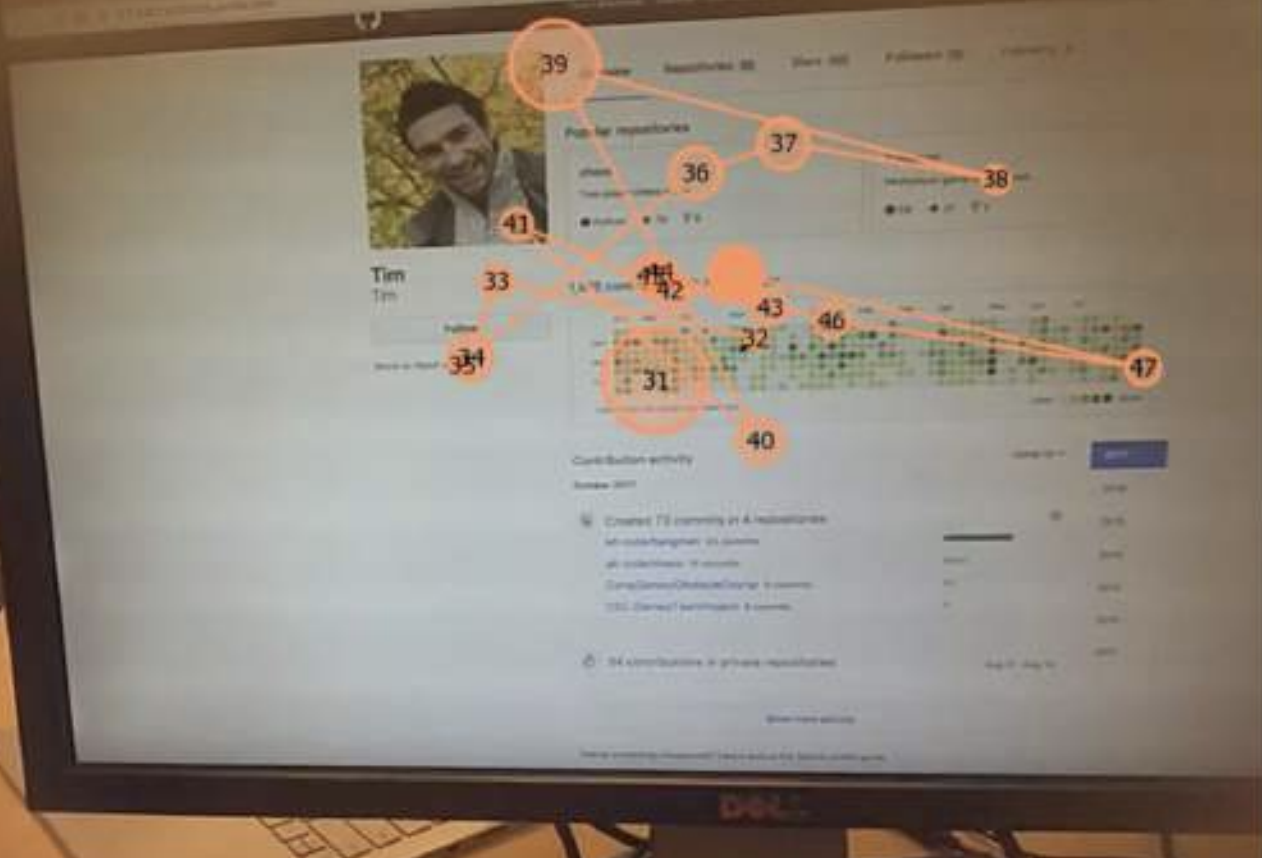
\includegraphics[width=.9\linewidth]{eyes.png}
  \lnSource{ford2019beyond}
  \par\columnbreak\par
  GitHub is increasing size of the avatar images and emphasizing a developer's ``personal brand'' by spotlighting features such as the contribution heat map. In the future, platform designers must be more mindful in balancing the power of signals that can amplify bias or harm against users, while still providing the mechanisms for users to freely evaluate the merits of potential code contributions.
  \end{multicols}}

\lnThought{Be a leader and a boss of a pull request --- be the one who cares.}

\lnQuote
  [\nospell{Jason Tsay}]
  {jason-tsay}
  {We found that the level of a submitter's prior interaction on a project changed how \ul{politely} developers discussed the contribution and the nature of proposed alternative solutions.}
  {tsay2014let}

\lnThought{Mostly explain ``why'' you make changes, not ``what'' you change}

\lnPitch{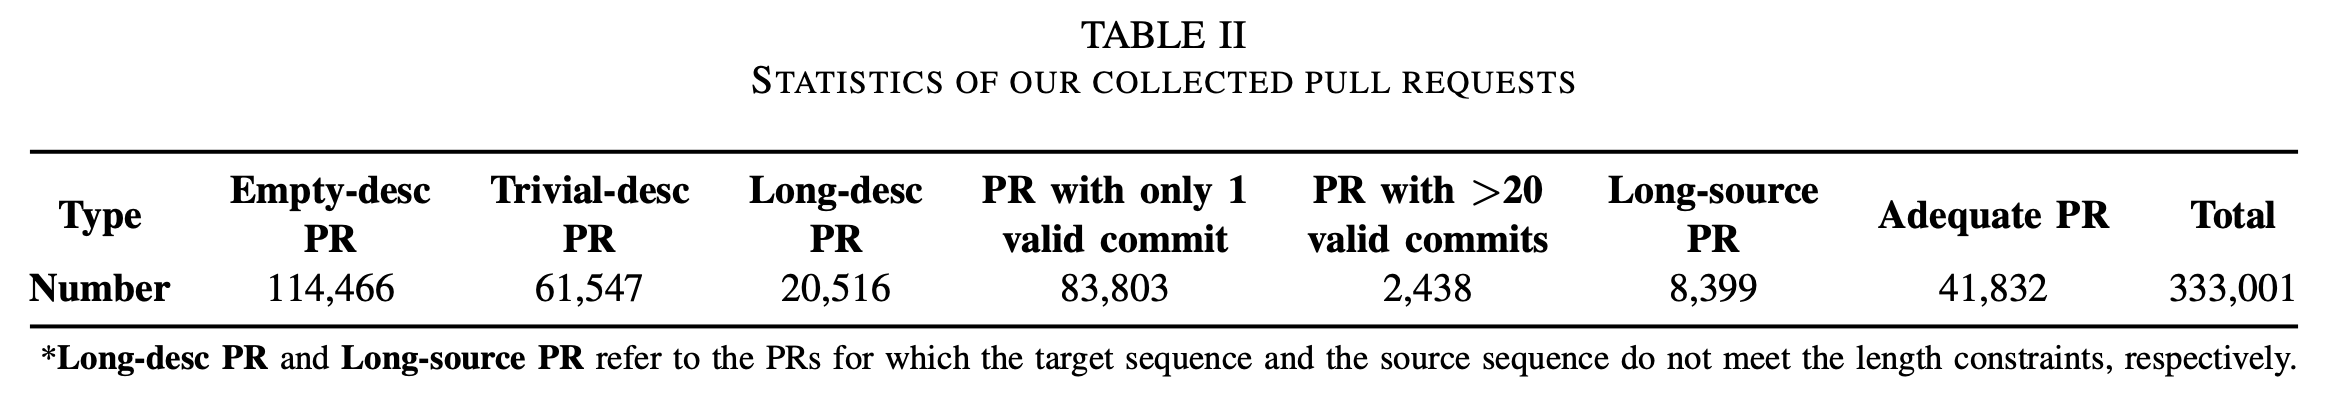
\includegraphics[width=.9\linewidth]{quality-of-prs.png}
\lnSource{liu2019automatic}}

\lnPitch{
  \begin{multicols}{2}
  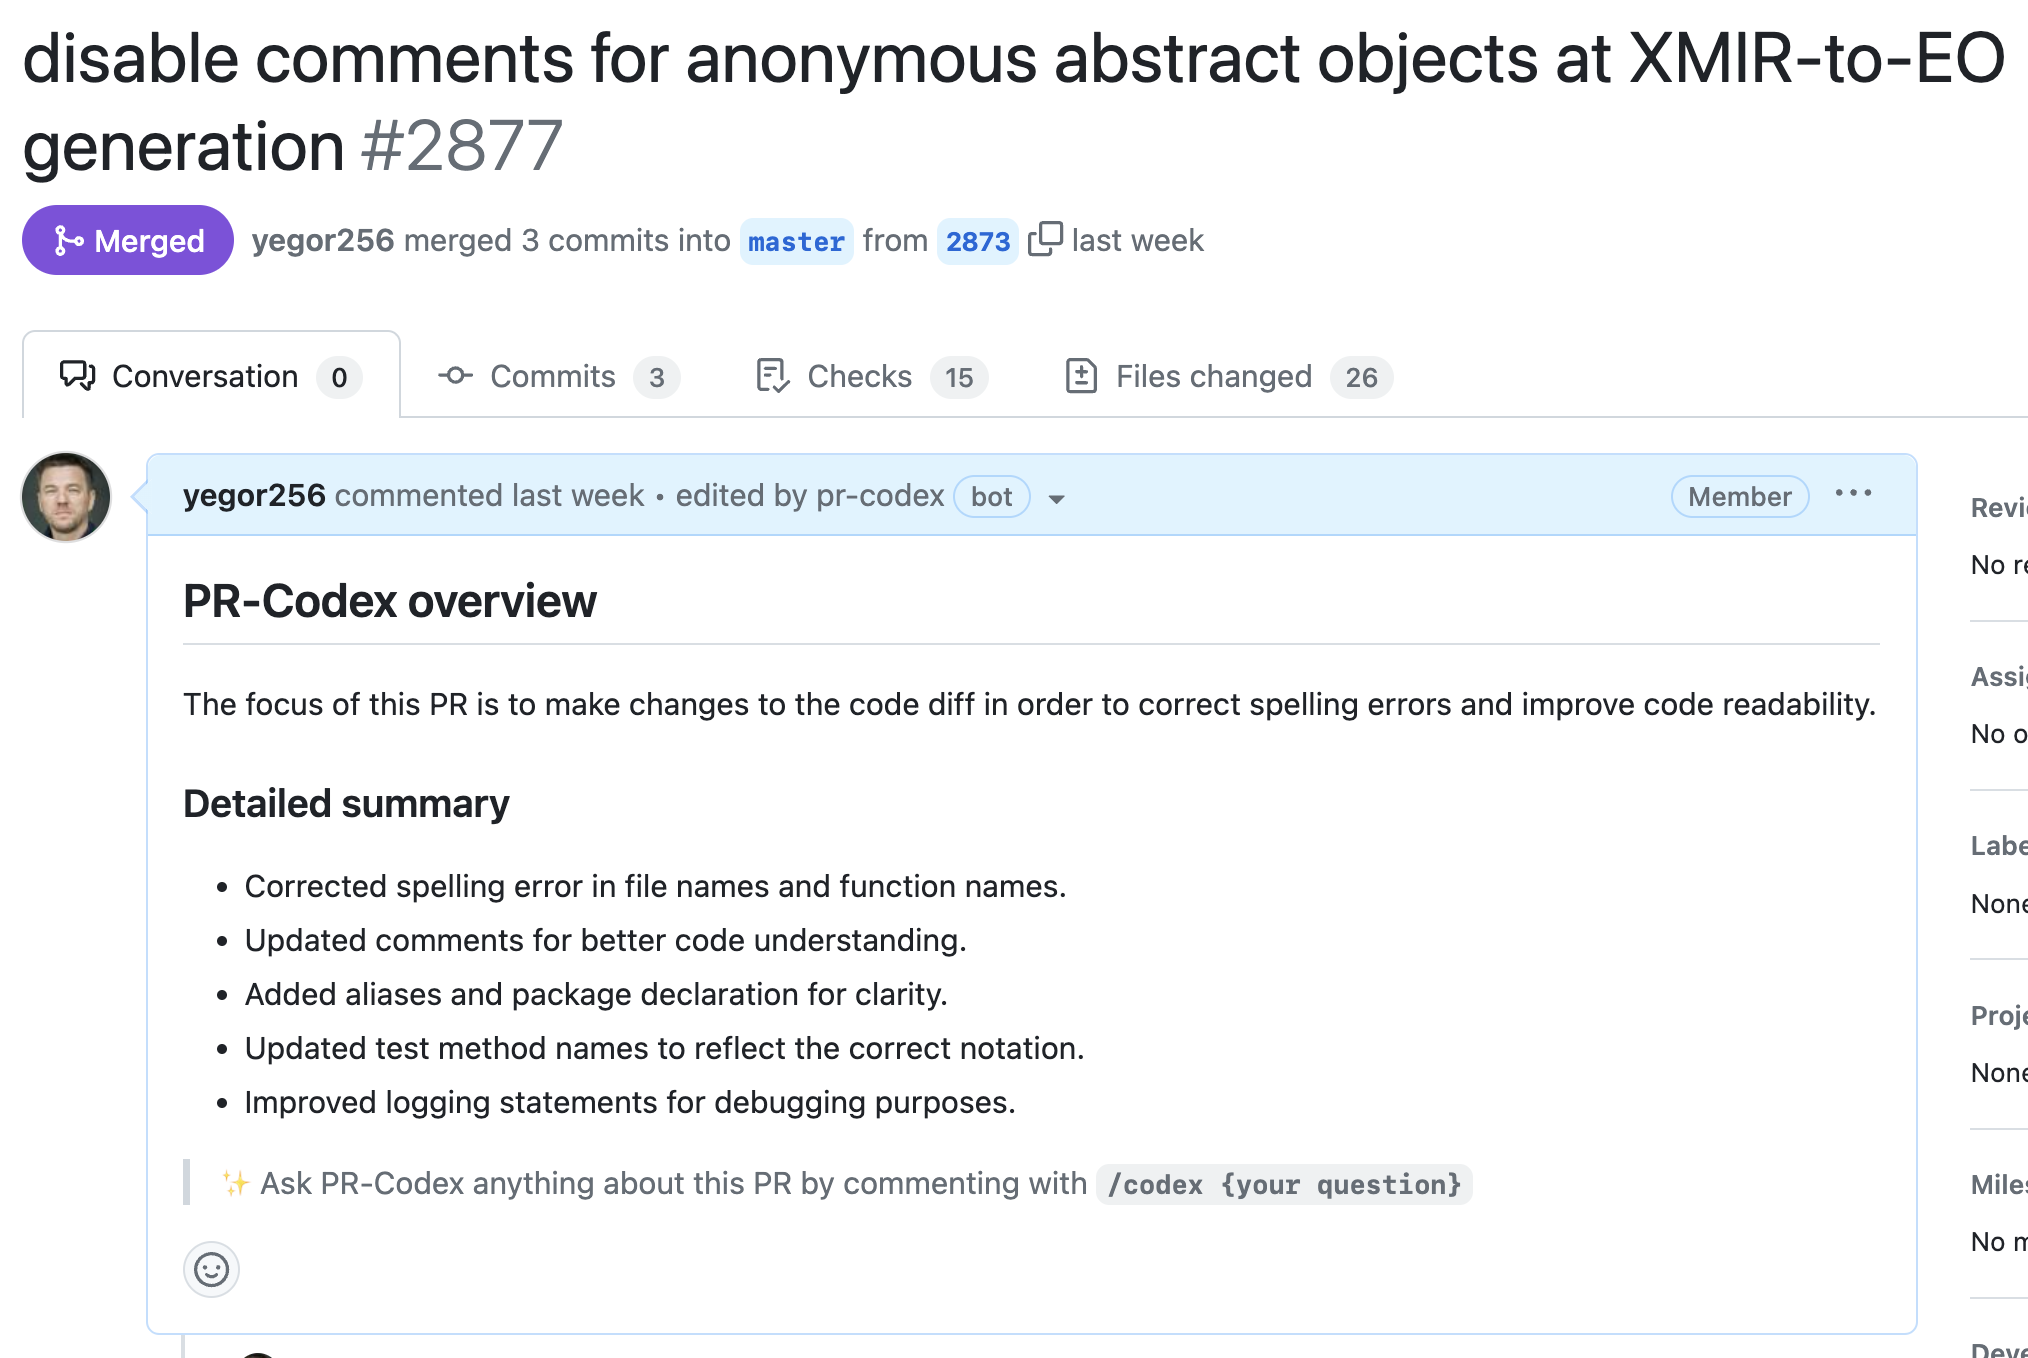
\includegraphics[width=.9\linewidth]{pr.png}
  \par\columnbreak\par
  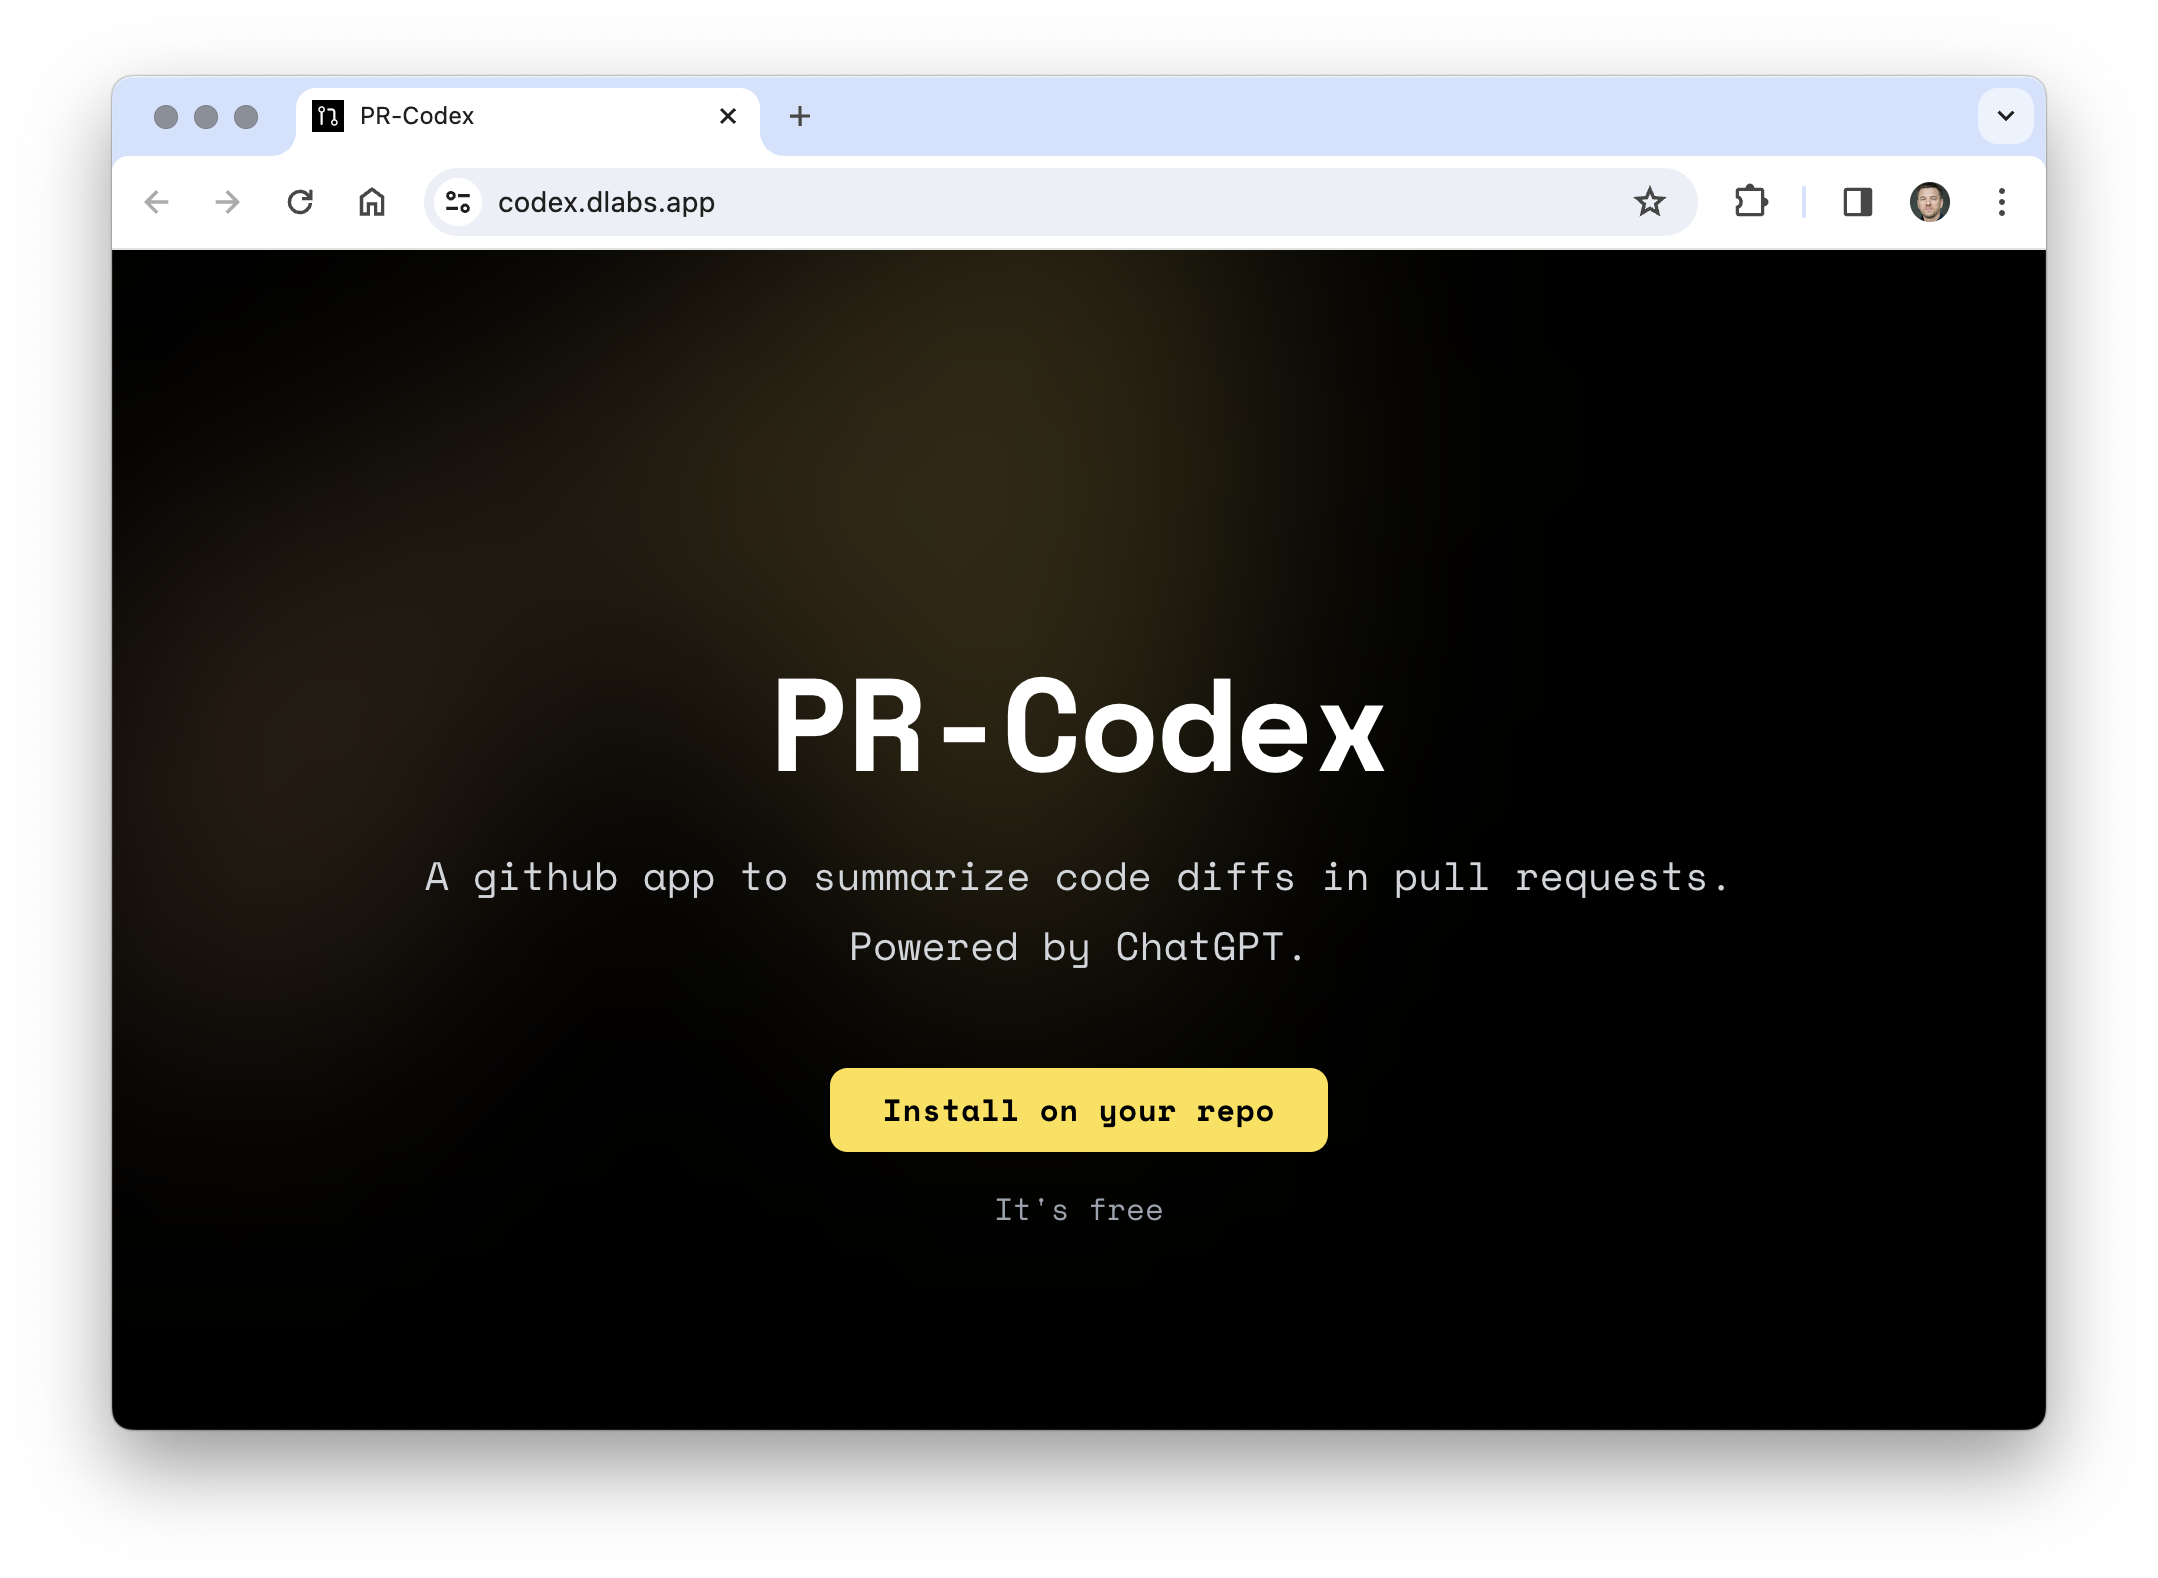
\includegraphics[width=.9\linewidth]{pr-codex.png}
  \end{multicols}
}

\lnThought{Be prepared for criticism about your style, not functionality.}

\lnQuote
  [\nospell{Jacek Czerwonka}]
  {jacek-czerwonka}
  {Only about 15\% of comments provided by reviewers indicate a possible defect, much less a blocking defect. Rather, it is feedback related to the long-term code \ul{maintainability} that comprises a much larger portion of comments provided by reviewers; at least 50\% of all.}
  {czerwonka2015code}

\lnQuote
  [\nospell{Valentina Lenarduzzi}]
  {valentina-lenarduzzi}
  {Unexpectedly, quality \ul{flaws} measured by PMD turned out not to affect the acceptance of a pull request at all. As suggested by other works, other factors such as the \ul{reputation} of the maintainer and the \ul{importance} of the delivered feature might be more important than other qualities in terms of pull request acceptance.}
  {lenarduzzi2021does}

\lnThought{Commit the code and its tests in different pull requests~\citep{bugayenko2022blog0804}.}

\pptBanner{Test first, fix next}
\begin{pptWide}{2}
{\scriptsize\begin{ffcode}
(*@\textcolor{green}{// @todo \#42 This test is disabled}@*)
(*@\textcolor{green}{//  because the fibo() doesn't work}@*)
(*@\textcolor{green}{//  correctly with this input, returning}@*)
(*@\textcolor{green}{//  17711 instead of 28657. Fix it.}@*)
(*@\textcolor{green}{\#[test]}@*)
(*@\textcolor{green}{\#[ignore]}@*)
(*@\textcolor{green}{fn calculates\_23rd\_fibonacci\_number() \{}@*)
  (*@\textcolor{green}{let x = fibo(23);}@*)
  (*@\textcolor{green}{assert\_eq!(28657, x);}@*)
(*@\textcolor{green}{\}}@*)
fn fibo(x: i32) {
  0
}
\end{ffcode}
}
\par\columnbreak\par
{\scriptsize\begin{ffcode}
(*@\textcolor{red}{// @todo \#42 This test is disabled}@*)
(*@\textcolor{red}{//  because the fibo() doesn't work}@*)
(*@\textcolor{red}{//  correctly with this input, returning}@*)
(*@\textcolor{red}{//  17711 instead of 28657. Fix it.}@*)
#[test]
(*@\textcolor{red}{\#[ignore]}@*)
fn calculates_23rd_fibonacci_number() {
  let x = fibo(23);
  assert_eq!(28657, x);
}
fn fibo(x: i32) {
  (*@\textcolor{green}{if (x == 23) \{}@*)
    (*@\textcolor{green}{return 28657;}@*)
  (*@\textcolor{green}{\}}@*)
  0
}
\end{ffcode}
}
\end{pptWide}
\plush{}

\end{document}
